%%%%%%%%%%%%%%%%%%%%%%%%%%%%%%%%%%%%%%%%%%%%%%%%%%%%%%%%%%%%%%%%%%%%
\section{Data Acquisition System (DAQ) Overview (Georgia Karagiorgi \& David Newbold)}
\label{sec:fdsp-daq-ov}

\metainfo{2 Pages - largely generic but some highlighting of SP-specifics.}

%%%%%%%%%%%%%%%%%%%%%%%%%%%%%%%%%
\subsection{Introduction}
\label{sec:fdsp-daq-intro}

The overall DUNE Far Detector Data Acquisition System (DAQ) is
illustrated in Fig.~\ref{fig:daq-overview}.
\fixme{Describe figure here.}

Figure.~\ref{fig:daq-overview} illustrates the data flow and the
exchange of trigger and monitoring messages.



\begin{dunefigure}[DAQ Overview]{fig:daq-overview}
  {A generalized overview of high-level far detector DAQ components showing one out of the four detector modules.  The electronics digitizes the detector signals and send the data to the DAQ Front-End Readout Hardware.  This component forms L0 Trigger Primitives and sends them and the data to a Front-End Computing Data Receiver.  The receiver sends the data to a RAM of sufficient size to buffer it longer than typical worse case trigger latency.  The L0 Trigger Primitives are forward to the Module Trigger Logic (MTL) unit which services the entire detector module.  The MTL forwards to the Global Trigger Logic unit which services the entire DUNE Far Detector.  Trigger commands are then sent back down and to the Event Builder Farm which, based on the trigger command information, queries the appropriate Front-End Computing units which return the requested data.  The Event Builder then aggregates the data and writes it to the Output Disk Buffer.  Each \SI{10}{\kton} module has specific differing details which are described below.}
% This PDF is made from the .dot of the same name.
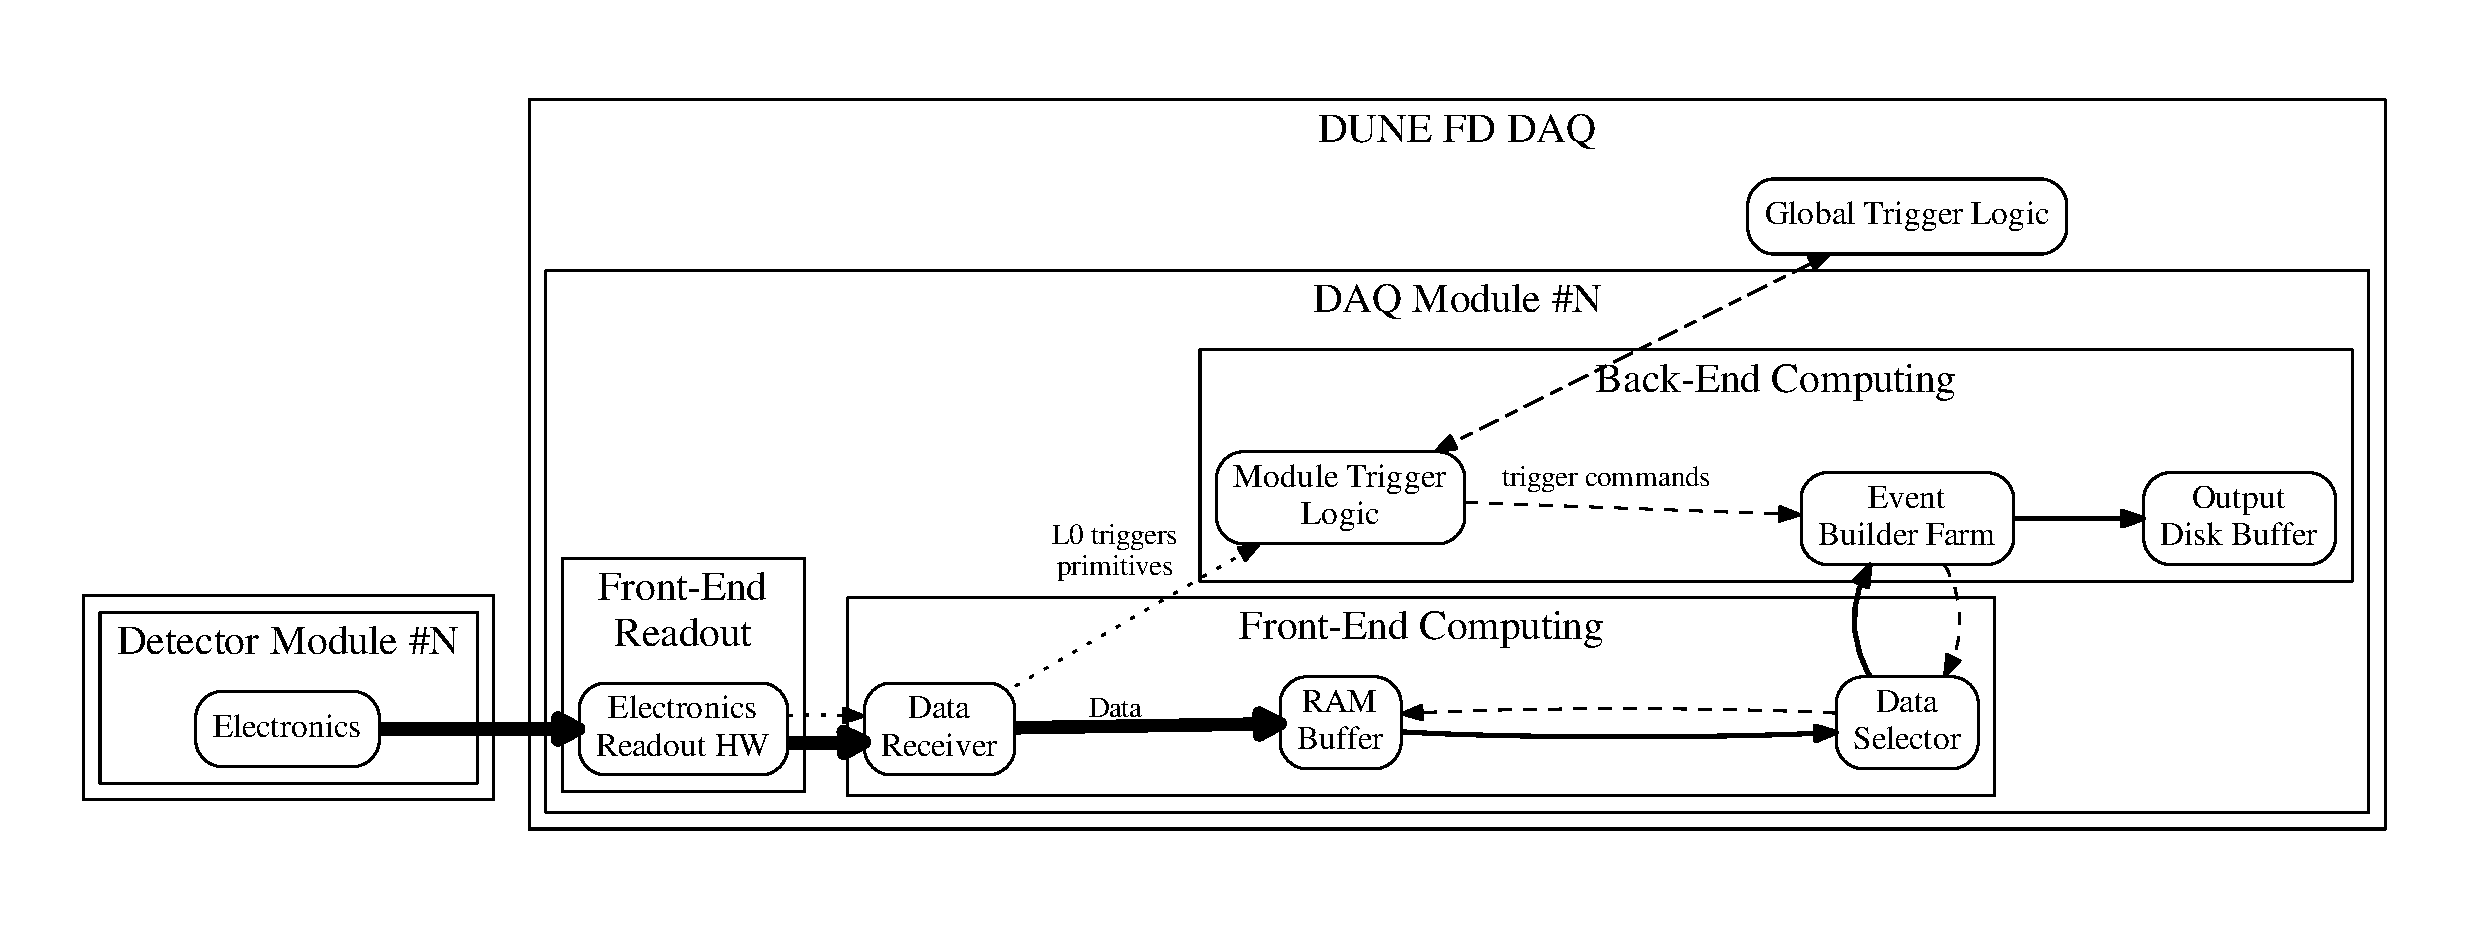
\includegraphics[width=0.8\textwidth]{daq-overview.pdf}%
\end{dunefigure}


%%%%%%%%%%%%%%%%%%%%%%%%%%%%%%%%%%%%%

\subsection{Design Considerations}
\label{sec:fdsp-daq-des-consid}


\metainfo{Include: Raw data rate from WIBs, Josh's table of data volumes for each event type and the 30 PB/year offline limit. Space and thermal power limits.  Note, this table may be better put into Section~\ref{sec:fdsp-daq-design} to make this section more generic.}


The Data Acquisition System design must enable... 
...

\fixme{Anne suggests: Within this section add ref to requirements document when it's ready, and maybe list the most important half dozen in a table here). E.g.,}  

\begin{dunetable}
[Important requirements on the DAQ system design]
{p{0.8\textwidth}}
{pdphysicsparams}
{Important requirements on the DAQ system design}   
Requirement  \\ \toprowrule
  \\ \colhline
   \\ \colhline
 ...\\ 
\end{dunetable}

\fixme{By the end of the volume, for every requirement listed in this section, there should exist an explanation of how it will be satisfied.}


%%%%%%%%%%%%%%%%%%%%%%%%%%%%%%%%
\subsection{Scope}
\label{sec:fdsp-daq-scope}

\metainfo{This section may also wish to refer to Fig.~\ref{fig:daq-overview}.}

The scope of the Data Acquisition System includes the continued procurement of materials for, and the fabrication, testing, delivery and installation of the following systems: 

\fixme{Whatever the items are...}

\begin{itemize}
\item Readout electronics 
\item 
\end{itemize}


\newpage 
